\documentclass[svgnames,11pt]{beamer}
\input{/home/tof/Documents/Cozy/latex-include/preambule_commun.tex}
\input{/home/tof/Documents/Cozy/latex-include/preambule_beamer.tex}
%\usepackage{pgfpages} \setbeameroption{show notes on second screen=left}
\author[]{Christophe Viroulaud}
\title{Système sur puce}
\date{\framebox{\textbf{Archi 18}}}
%\logo{}
\institute{Terminale - NSI}
\begin{document}
\begin{frame}
\titlepage
\end{frame}
\begin{frame}
    \frametitle{}

    En 1975, Gordon Moore prédit la conjecture suivante:
    \begin{center}
        \emph{Le nombre de transistors sur une puce va doubler tous les deux ans.}
    \end{center}
    \note[item]{cofondateur Intel}
    \note[item]{revu: tous les 18 mois}
\end{frame}
\begin{frame}
    \frametitle{}

    \begin{center}
        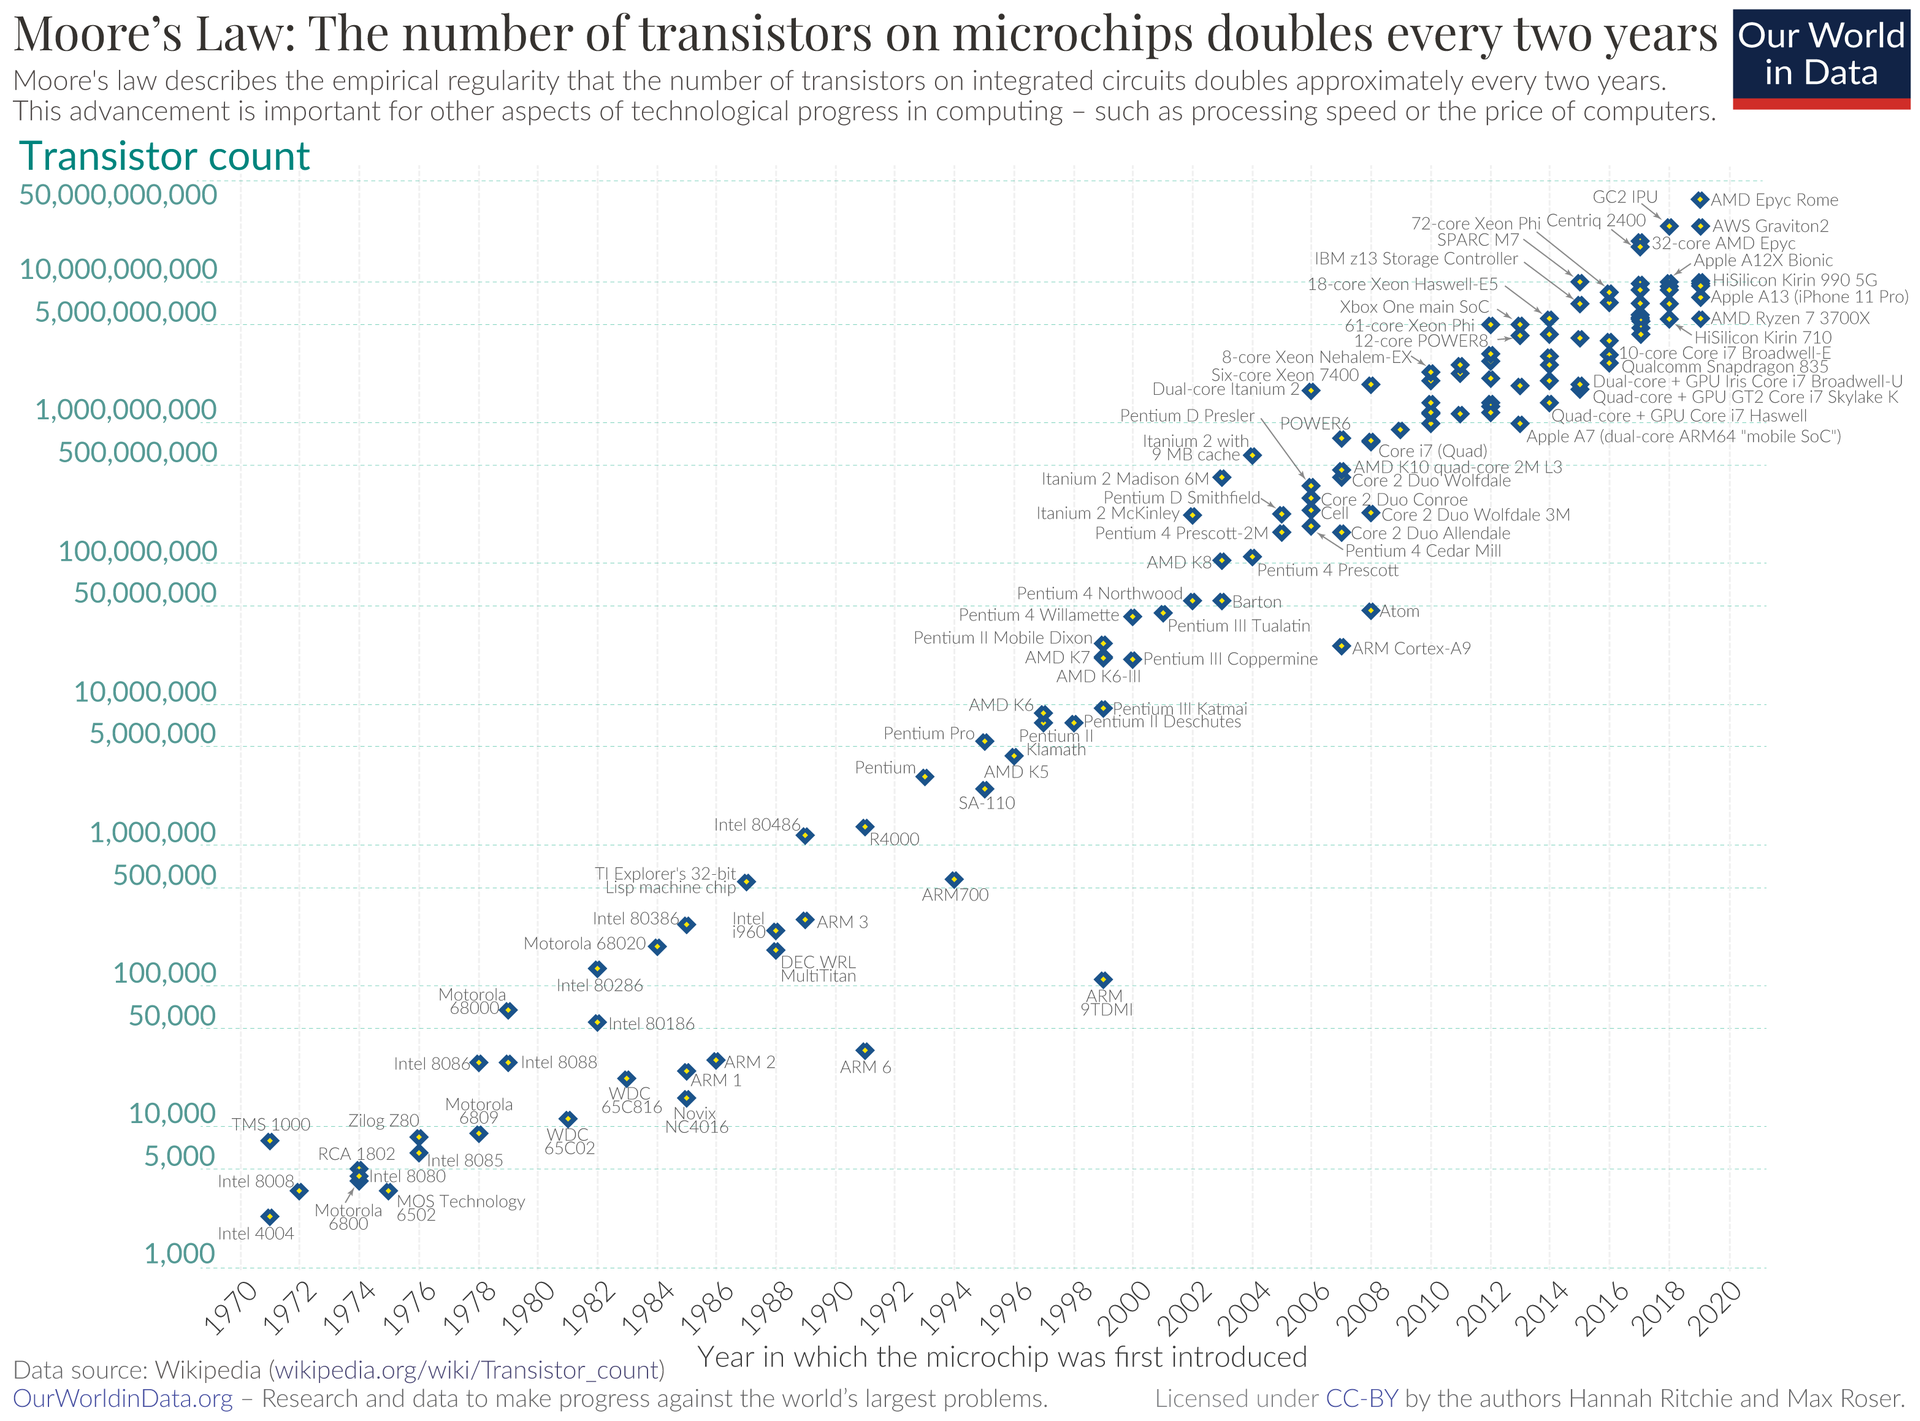
\includegraphics[width=10cm]{ressources/moore.png}
    \end{center}

\end{frame}
\begin{frame}
    \frametitle{}

    \begin{framed}
        \centering Qu'est-ce qu'un système sur puce?
    \end{framed}

\end{frame}
\section{Évolution de l'informatique}
\begin{frame}
    \frametitle{Évolution de l'informatique}
\begin{aretenir}[Rappels]
On place souvent l'avènement du premier ordinateur à la fin de la seconde guerre mondiale. John von Neumann en décrit les principes en 1946. Ces machines utilisaient à l'époque des tubes électroniques -ou tubes à vide. L'invention du transistor en 1947 et son utilisation dans les ordinateurs dès 1950 permit de réaliser de grandes avancées.
\end{aretenir}
    

\end{frame}
\begin{frame}
    \frametitle{}

    \begin{activite}
    \begin{enumerate}
        \item Rappeler le principe de l'architecture de von Neumann.
        \item Qu'est-ce qu'un circuit intégré? Quand est-il inventé?
        \item À quelle date apparaissent les microprocesseurs?
        \item L'Intel 4004 est considéré comme un des premiers modèles commerciaux. Quelles étaient ses performances?
        \item Quelles sont les performances actuelles des microprocesseurs?
    \end{enumerate}
    \end{activite}
\note[item]{1958: circuit intégré}
\note[item]{1969: microprocesseur}
\note[item]{1971: intel 4004 2250 transistors, 60000 opérations /s}
\note[item]{aujourd'hui: plusieurs milliards; 1Ghz = $10^9$ opérations par seconde}
\end{frame}
\section{Microcontrôleur}
\begin{frame}
    \frametitle{Microcontrôleur}

    \begin{aretenir}[]
    Un microcontrôleur est un circuit intégré, dédié à une tâche spécifique. Ils peuvent être assimilés à des \emph{mini-ordinateurs} mais avec une puissance bien moindre.\\Ils sont principalement utilisés dans les systèmes embarqués. Une voiture peut, par exemple, regrouper jusqu'à 50 microcontrôleurs (régulateur de vitesse, détecteur de pluie\dots)
    \end{aretenir}

\end{frame}
\begin{frame}
    \frametitle{}

    \begin{activite}
    \begin{enumerate}
        \item Quels sont les composants qu'on retrouve sur un microcontrôleur?
        \item Qu'est-ce qu'un \emph{bus} en informatique?
        \item Si la taille d'un mot mémoire est de 16 bits, quelle est la taille du bus adéquate?
        \item Expliquer brièvement l'architecture de \emph{Harvard} et ses différences avec celle de von Neumann.
        \item Quels sont les avantages de ces composants?
    \end{enumerate}
    \end{activite}
\note[item]{CPU, mémoire (programme et données), entrées/sorties}
\note[item]{fréquence horloge beaucoup plus faible, et mémoire plus petite (qq ko) $\rightarrow$ moins puissant mais moins énergivore}
\note[item]{Harvard: séparation mémoire programme et données; d'où séparation des bus également $\rightarrow$ simplifications; jeu d'instructions réduites: RISC (Reduced Instruction Set Computer)}
\end{frame}
\section{Système sur puce}
\begin{frame}
    \frametitle{Système sur puce}

    \begin{aretenir}[]
        La miniaturisation des transistors permet de rassembler dans les systèmes sur puce (\emph{Soc} System on Chip), tous les composants habituellement présents sur la carte mère d'un ordinateur. Leur architecture et leurs caractéristiques sont de fait très proches de celles d'un ordinateur classique. Une différence notable cependant est la longueur des bus qui est drastiquement diminuée dans un circuit intégré.
    \end{aretenir}
\note[item]{fréquence d'horloge similaire à celles d'un PC}
\end{frame}
\begin{frame}
    \frametitle{}

    \begin{center}
    \centering
    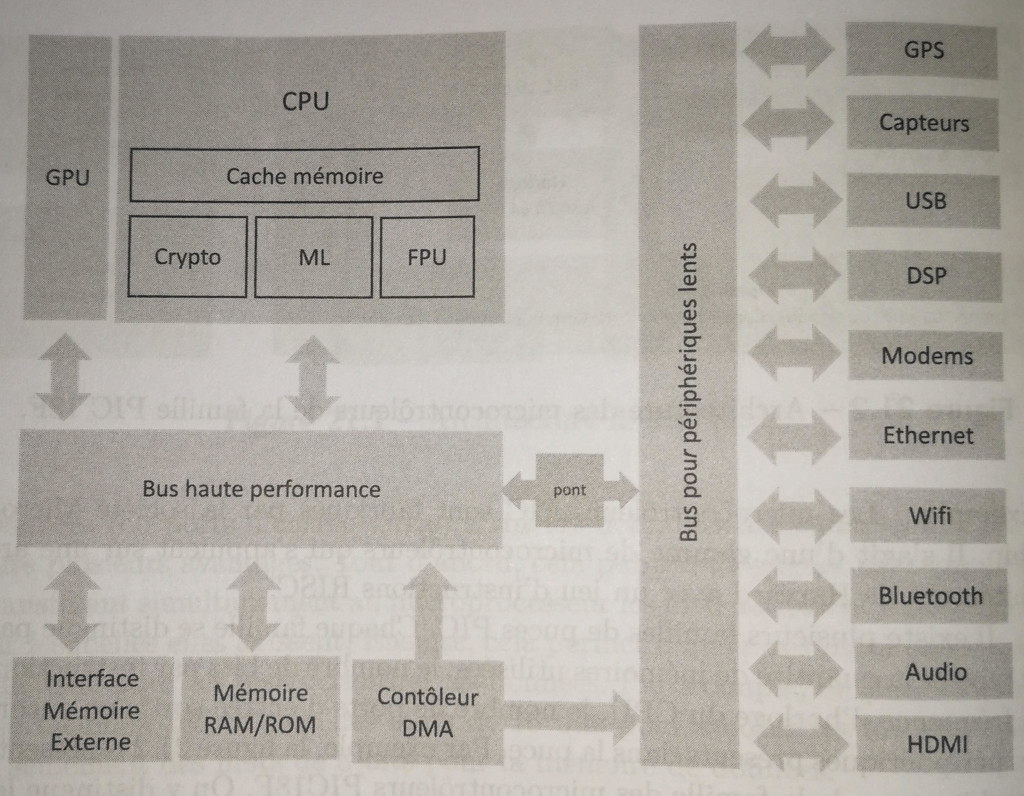
\includegraphics[width=10cm]{ressources/soc.jpg}
    \captionof{figure}{Architecture d'un système sur puce}
    \label{IMG}
    \end{center}

\end{frame}
\begin{frame}
    \frametitle{}

    Le CPU peut contenir des circuits dédiés à certaines opérations:
    \begin{itemize}
        \item Quel rôle joue la fréquence d'horloge dans un CPU?
        \item FPU: Floating Point Unit
        \item ML: Machine Learning
        \item Crypto: Unité qui implémente des opérations élémentaires pour accélérer les algorithmes cryptographiques.
    \end{itemize}
\note[item]{fréquence: nb instructions par seconde}
\end{frame}
\begin{frame}
    \frametitle{}

    \begin{center}
        \includegraphics[width=10cm]{ressources/raspberry.jpg}
        \captionof{figure}{\centering Le Raspberry est un ordinateur basé sur un SoC. Le système sur puce est le carré argenté au centre.}
    \end{center}

\end{frame}
\begin{frame}
    \frametitle{}
\begin{center}
\centering
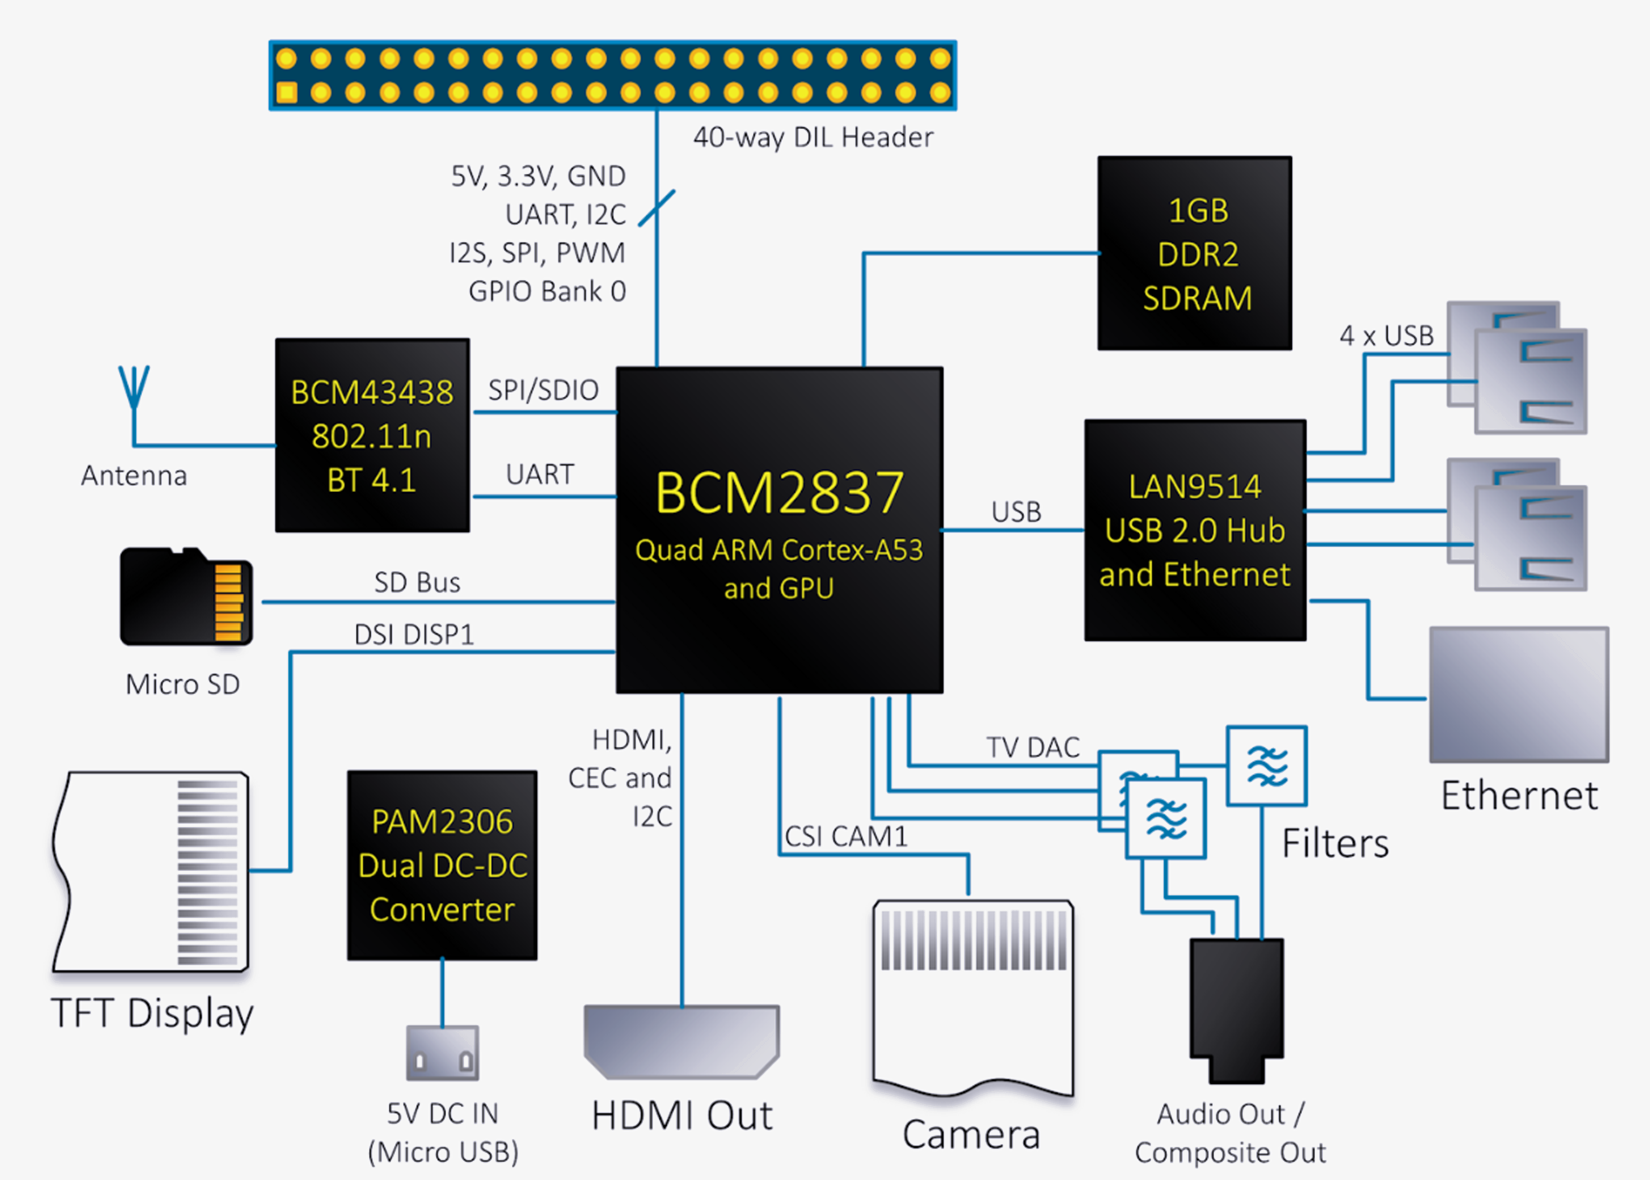
\includegraphics[width=10cm]{ressources/raspberry-schema.png}
\captionof{figure}{\centering Schéma du Raspberry}
\label{IMG}
\end{center}

\end{frame}
\begin{frame}
    \frametitle{}

    \begin{activite}
    \begin{enumerate}
        \item Sur un Raspberry, si le SoC est seulement la partie centrale, qu'est-ce que sont tous les composants autour?
        \item Quel est le rôle du contrôleur DMA?
        \item Quel est l'avantage d'avoir des longueurs de bus réduites?
        \item Qu'est-ce que le Machine Learning?
        \item Quels appareils du quotidien sont basés sur un SoC?
        \item Quels sont les avantages et les inconvénients des SoC?
    \end{enumerate}
    \end{activite}
\note[item]{bus réduit: plus rapide et moins de chaleur dégagée $\rightarrow$ pas de ventilateur}
\note[item]{DMA: Direct Memory Access: transfert directement données de la mémoire vers périphériques, sans passer par CPU}
\note[item]{avantages: énergie, coût, sécurité (pas de possibilité de modification)}
\note[item]{inconvénient: pas de possibilité de modif: un transistor out et il faut tout changer}
\end{frame}
\begin{frame}
    \frametitle{}

    Dans un SoC, le CPU est cadencé à une fréquence tellement élevée, que toutes les opérations de lecture/écriture ralentissent fortement sont travail.
    \begin{activite}
    Quel composant, placé proche du CPU, permet de compenser ce ralentissement. Donner une brève explication de son fonctionnement.
    \end{activite}
\note[item]{cache mémoire}
\end{frame}
\end{document}